%%%%%%%%%%%%%%%%%%%%%%%%%%%%%%%%%%%%%%%%%%%%%%%%%%%%%%%%%%%%%%%%%%%%%
%
%  This is a sample LaTeX input file for your contribution to 
%  the MC2013 conference. Modified by R.C. Martineau at INL from A. 
%  Sood at LANL, from J. Wagner ORNL who obtained the original class 
%  file by Jim Warsa, LANL, 16 July 2002}
%
%  Please use it as a template for your full paper 
%    Accompanying/related file(s) include: 
%       1. Document class/format file: mc2013.cls
%       2. Sample Postscript Figure:   figure.eps
%       3. A PDF file showing the desired appearance: template.pdf 
%    Direct questions about these files to: richard.martinea@inl.gov
%
%    Notes: 
%      (1) You can use the "dvips" utility to convert .dvi 
%          files to PostScript.  Then, use either Acrobat 
%          Distiller or "ps2pdf" to convert to PDF format. 
%      (2) Different versions of LaTeX have been observed to 
%          shift the page down, causing improper margins.
%          If this occurs, adjust the "topmargin" value in the
%          mc2013.cls file to achieve the proper margins. 
%
%%%%%%%%%%%%%%%%%%%%%%%%%%%%%%%%%%%%%%%%%%%%%%%%%%%%%%%%%%%%%%%%%%%%%


%%%%%%%%%%%%%%%%%%%%%%%%%%%%%%%%%%%%%%%%%%%%%%%%%%%%%%%%%%%%%%%%%%%%%
\documentclass{mc2013}
%
%  various packages that you may wish to activate for usage 
\usepackage{graphicx}
\usepackage{tabls}
\usepackage{afterpage}
\usepackage{cites}
%\usepackage{epsf}
\usepackage{amssymb}
\usepackage{amsmath}
% more math
\usepackage{amsfonts}
\usepackage{amssymb}
\usepackage{amstext}
\usepackage{amsbsy}
\usepackage{array}
\usepackage{xspace}
\usepackage{color}
\usepackage{graphicx}
\usepackage{float} % utiliser H pour forcer a mettre l'image ou on veut
\usepackage{lscape} % utilisation du mode paysage
\usepackage{mathbbol} % permet d'avoir le vrai symbol pour les reels grace a mathbb
\usepackage{enumerate} % permet d'utiliser enumerate
%\usepackage{marvosym} % permet d'avoir le symbol pour le nucleaire
\usepackage{moreverb} % permet d'utiliser verbatimtab : conservation la tabulation
\usepackage{stmaryrd} % permet d'utiliser \llbrackedt et \rrbracket : double crochet
\usepackage{caption}
\usepackage{subcaption}
\usepackage[noabbrev]{cleveref} % permet d'utiliser cref and Cref



\newcommand\bn{\boldsymbol{\nabla}}
\newcommand\bo{\boldsymbol{\Omega}}
\newcommand\br{\mathbf{r}}
\newcommand\la{\left\langle}
\newcommand\ra{\right\rangle}
\newcommand\bs{\boldsymbol}
\newcommand\red{\textcolor{red}}
\newcommand\blue{\textcolor{blue}}
\newcommand\ldb{\{\!\!\{}
\newcommand\rdb{\}\!\!\}}
\newcommand\llb{\llbracket}
\newcommand\rrb{\rrbracket}
\newcommand{\jmp}[1]{[\![#1]\!]}                     % jump
\newcommand{\mvl}[1]{\{\!\!\{#1\}\!\!\}}             % mean value

\newcommand\tf{\varphi}

\newcommand\mc{\mathcal}

\renewcommand{\(}{\left(}
\renewcommand{\)}{\right)}
\renewcommand{\[}{\left[}
\renewcommand{\]}{\right]}
\newcommand{\sn}{\ensuremath{S_n}\xspace}
\newcommand{\eqt}[1]{Eq.~(\ref{#1})}                     % equation
\newcommand{\fig}[1]{Fig.~\ref{#1}}                      % figure
\newcommand{\tbl}[1]{Table~\ref{#1}}                     % table
%
% Insert authors' names and short version of title in lines below
%
\newcommand{\authorHead}      % Author's names here
   {Bruno Turcksin, Jean C. Ragusa}  
\newcommand{\shortTitle}      % Short title here
   {A DSA Scheme For Rectangular Geometries Based On BLD Finite Elements}  
%%%%%%%%%%%%%%%%%%%%%%%%%%%%%%%%%%%%%%%%%%%%%%%%%%%%%%%%%%%%%%%%%%%%%
%
%   BEGIN DOCUMENT
%
%%%%%%%%%%%%%%%%%%%%%%%%%%%%%%%%%%%%%%%%%%%%%%%%%%%%%%%%%%%%%%%%%%%%%
\begin{document}

%
%      Headers and Footers
\afterpage{%
\fancyhf{}%
\fancyhead[CE]{              
{\scriptsize \authorHead}}                                                
\fancyhead[CO]{               
{\scriptsize \shortTitle}}                  
%\lfoot{\scriptsize{
%International Conference on Mathematics and Computational Methods
%Applied to Nuclear Science \& Engineering (M\&C 2013), 
%\\ Sun Valley, Idaho, USA, May 5-9, 2013.}}%
\rfoot{\thepage/\totalpages{}}%

\pagestyle{fancy}
%\setlength{\topmargin}{-20pt}
}
 
\normalsize

\setlength{\baselineskip}{16.8pt}
\vspace{-3pt}

% 
% TITLE
%

\begin{center}
\textbf{\large %
%A BI-LINEAR DISCONTINUOUS FINITE ELEMENT DIFFUSION SYNTHETIC ACCELERATION IN RECTANGULAR GEOMETRIES \\
A DIFFUSION SYNTHETIC ACCELERATION SCHEME FOR RECTANGULAR GEOMETRIES BASED ON BILINEAR DISCONTINUOUS FINITE ELEMENTS\\
}
% 
% FIRST AUTHORS 
%
\setlength{\baselineskip}{14pt}
\textbf{Bruno Turcksin and Jean C. Ragusa}\footnote{Corresponding author} \\
Department of Nuclear Engineering \\
Texas A\&M University  \\
bruno.turcksin@neo.tamu.edu; jean.ragusa@tamu.edu \\

% 
%% SECOND AUTHORS (if not needed delete from here) 
%%
%\vspace{12pt}
%\textbf{Double space and list Author C}\\
%Department of Nuclear Engineering  \\
%Name of University \\
%Address \\
%C@name.univ.edu\\ 
%%
%% SECOND AUTHORS (to here)
%%

\end{center}

%
% SET RAGGED RIGHT MARGIN
%
\raggedright


\section*{ABSTRACT} 
\begin{quote}
\begin{small}
A DSA technique to accelerate the iterative convergence of \sn transport solves is derived for bilinear discontinuous (BLD) finite elements on rectangular grids.
The diffusion synthetic acceleration equations are discretized using BLD elements by adapting the Modified Interior Penalty technique, introduced 
in \cite{mip} for triangular grids. The MIP-DSA equations are SPD and thus are solved using a preconditioned CG technique. Fourier analyses and implementation of the technique in a BLD \sn transport code show that the technique is stable is effective. 

\emph{Key Words}: diffusion synthetic acceleration (DSA), bilinear discontinuous finite element (BLD)
\end{small} 
\end{quote}

\setlength{\baselineskip}{14pt}
\normalsize

%%%%%%%%%%%%%%%%%%%%%%%%%%%%%%%%%%%%%%%%%%%%%%%%%%%%%%%%%%%%%%%%%%%%%%%%%%%%%%%%%%%%%%
%%%%%%%%%%%%%%%%%%%%%%%%%%%%%%%%%%%%%%%%%%%%%%%%%%%%%%%%%%%%%%%%%%%%%%%%%%%%%%%%%%%%%%
\Section{INTRODUCTION} 
%%%%%%%%%%%%%%%%%%%%%%%%%%%%%%%%%%%%%%%%%%%%%%%%%%%%%%%%%%%%%%%%%%%%%%%%%%%%%%%%%%%%%%
%%%%%%%%%%%%%%%%%%%%%%%%%%%%%%%%%%%%%%%%%%%%%%%%%%%%%%%%%%%%%%%%%%%%%%%%%%%%%%%%%%%%%%

The Discontinuous Finite Element Method (DFEM) is a common spatial discretization technique for 
the discrete-ordinate (\sn) transport equations. 
The scattering source is usually converged using either a Richardson method, i.e., the Source Iteration (SI) technique,
or a Krylov subspace approach (typically GMRes). 
For highly diffusive materials in optically thick configurations, these iterative techniques 
can become quite ineffective, requiring high iteration counts.
However, SI and GMRes-based transport solves 
can be accelerated (preconditioned) with DSA approaches \cite{dsa_ref},
leading to preconditioned Richardson and preconditioned GMRes versions, respectively.
%However, both SI and GMRes can become inefficiently 
%thick diffusive configurations. For isotropic (and weakly anisotropic) scattering, a Diffusion
%Synthetic Acceleration (DSA) technique, leading to preconditioned Richardson and preconditioned GMRes versions, respectively,
%can significantly reduce .
%
Yet, it is also well established that the spatial discretization of the DSA equations
must be ``consistent'' with the one used for the \sn transport equations to
yield unconditionally stable and efficient DSA schemes
(\cite{dsa_ref,larsen_dsa,consistent_p1,wla,mip}). However, the search for full
consistency between the discretized transport equations and the discretized
diffusion may not be computationally practical \cite{consistent_p1} and 
some partially consistent DSA schemes have been analyzed for DFE discretizations 
of the transport (e.g., \cite{wla,mip}).

Here, we present a bilinear discontinuous (BLD) finite element technique for the DSA equations.
That is, the same spatial discretization is employed for both the \sn transport equation and the diffusion 
synthetic accelerator. There are
several advantages for using the same finite element space in both discretizations: 
(a) many of the elementary matrices employed to discretize the
transport operator are also used for the discretization of the DSA operator; 
(b) should a continuous finite element discretization (as in the case of the WLA method \cite{wla}, for instance),
be chosen to discretize the DSA equations on spatially adapted meshes, hanging nodes treatment is required 
in order to preserve the continuous nature of finite element solution; however, a discontinuous discretization 
would deal seamlessly with spatially adapted meshes. Our BLD discretization of the DSA equations is an extension of
the MIP method, introduced in \cite{mip} for triangular meshes.

The remainder of the paper is as follows. In Section~\ref{sec:ip}, we recall some of the traditional 
discontinuous finite element approximations utilized to solve the diffusion equation and present the symmetric
interior penalty scheme. The SI and GMRes solution techniques for the
\sn transport equations are briefly given in Section~\ref{sec:transport}. In Section~\ref{sec:mip}, the DSA equations
for the Modified Interior Penalty (MIP) are given in the case of a bilinear discontinuous discretization. Fourier
analyses and numerical results are presented in Section~\ref{sec:results}. We conclude and 
propose extensions to this work in Section~\ref{sec:ccl}.


%%%%%%%%%%%%%%%%%%%%%%%%%%%%%%%%%%%%%%%%%%%%%%%%%%%%%%%%%%%%%%%%%%%%%%%%%%%%%%%%%%%%%%
%%%%%%%%%%%%%%%%%%%%%%%%%%%%%%%%%%%%%%%%%%%%%%%%%%%%%%%%%%%%%%%%%%%%%%%%%%%%%%%%%%%%%%
\Section{DISCONTINUOUS FINITE ELEMENT DISCRETIZATIONS FOR THE DIFFUSION EQUATION} \label{sec:ip}
%%%%%%%%%%%%%%%%%%%%%%%%%%%%%%%%%%%%%%%%%%%%%%%%%%%%%%%%%%%%%%%%%%%%%%%%%%%%%%%%%%%%%%
%%%%%%%%%%%%%%%%%%%%%%%%%%%%%%%%%%%%%%%%%%%%%%%%%%%%%%%%%%%%%%%%%%%%%%%%%%%%%%%%%%%%%%

Discontinuous finite element approximations are well-established for elliptic equations; see, for
instance, \cite{Kanschat2007}. The interior penalty family of methods has its origin in Nitsche's weak enforcement
of Dirichlet boundary conditions \cite{nitsche}: rather than imposing that the numerical solution be equal to the
user-specified boundary value, Nitsche proposed to add the following term (appropriately weighted) 
in the weak formulation $\int_{\partial V} (\Phi^{Dir}-\Phi)^2$; 
here, $\Phi^{Dir}$ denotes the Dirichlet boundary value, $\Phi$ is the numerical 
solution, $\partial \mc{D}$ is the boundary of the computational domain $\mc{D}$. Later, the idea was extended to
include any ``interior interface'' (i.e., interfaces between cells). Many variants of interior penalty methods have
been derived over the years (see the review articles \cite{Kanschat2007,ip-review}). Below, we briefly
recall the symmetric interior penalty technique applied to diffusion equation. In Section~\ref{sec:mip},
this technique will be slightly modified for use as a diffusion synthetic accelerator.
%
%
Consider the following diffusion problem :
\begin{equation}
  -\bn \cdot D \bn \phi + \Sigma_a \phi = Q_0\ \textrm{ for } (x,y) \in \mc{D}=[0,L_x]\times[0,L_y],
\end{equation}
\begin{equation}
%  \phi = \phi^D \ \textrm{ for } (x,y) \in \partial \mc{D}.
\frac{1}{4}\phi - \frac{1}{2} D \partial_n \phi =J^{inc}\ \textrm{ for } (x,y) \in \partial \mc{D}.
\end{equation}
%
where $D$ is the diffusion coefficient, $\phi$ is the scalar flux, $\Sigma_a$
is the absorption cross section, $Q_0$ is a volumetric source, $J^{inc}$ is an
incoming current value. The weak form for the symmetric interior penalty is given by (see, e.g., \cite{Kanschat2007}):
\begin{equation}
\label{eq:ip-form}
  b_{IP}(\phi,\tf) = l_{IP}(\tf),
\end{equation}
where the bilinear form is:
\begin{equation}
\label{eq:matrix-ip-form}
  \begin{split}
    b_{IP} (\phi,\tf) =& \(D\bn\phi,\bn \tf\)_{\mc{T}_h} + \(\Sigma_a \phi,\tf\)_{\mc{T}_h}  +
    (\kappa_e^{IP}\jmp{\phi},\jmp{\tf})_{E_h^i}\\
    &+ \( \jmp{\phi}, \mvl{D\partial_n \tf}\)_{E_h^i}
     + \( \jmp{\tf}, \mvl{D\partial_n \phi}\)_{E_h^i} \\
    &+ \(2\kappa_e^{IP} \phi, \tf \)_{\partial \mc{D}}
    -\frac{1}{2}\(\phi,D\partial_n \tf\)_{\partial \mc{D}}
    -\frac{1}{2}\(D\partial_n\phi,\tf\)_{\partial \mc{D}}
  \end{split}
\end{equation}
and the linear form is:
\begin{equation}
\label{eq:rhs-ip-form}
  l_{IP}(\tf) = \(Q_0,\tf\)_{\mc{T}_h} + (J^{inc},\tf)_{\partial \mc{D}},
\end{equation}
%
%
where $\mc{T}_h$ is the mesh used to discretize $\mc{D}$ into non-overlapping 
elements $K$, such that the union of the elements fully covers $\mc{D}$, $E_h^i$ is 
the set of interior edges such that $E_h^i= \cup _{K_1,K_2\in \mc{T}_h}(\partial K_1 \cap \partial K_2)$,
and $\tf$ a bilinear discontinuous basis function. These BLD functions, given for the cell spanning 
$[0,{\Delta x}]\times[0, \Delta y]$, are:
\begin{align*}
& \tf_1 = \frac{{\Delta x}-x}{{\Delta x}}\frac{\Delta y-y}{\Delta y}\\
& \tf_2 = \frac{x}{{\Delta x}} \frac{\Delta y-y}{\Delta y}\\
& \tf_3 = \frac{x}{{\Delta x}}\frac{y}{\Delta y}\\
& \tf_4 = \frac{{\Delta x}-x}{{\Delta x}}\frac{y}{\Delta y}
\end{align*}
We also have defined the jump and mean values as:
\begin{equation}
  \jmp{\phi} = \phi^+ - \phi^-,\quad
  \mvl{\phi} =  \frac{\phi^++\phi^-}{2}.
\end{equation}
The penalty parameter $\kappa_e^{IP}$ is given:
\begin{equation}
\label{eq:penalty-ip}
  \kappa_e^{IP} = \left\{
    \begin{aligned}
      & \frac{C}{h_{\bot}} \frac{D^+ +D^-}{2} & \textrm{ on interior edges, i.e., } e \in  E_h^i,\\
      & C\frac{D}{h_{\bot}} & \textrm{ on boundary edges, i.e., } e \in \partial \mc{D},
    \end{aligned}
    \right.
\end{equation}
where $C$ is a constant (we used $C=2$) and $h_{\bot}$ is the
length of the cell in the direction orthogonal to edge $e$.  The $+$ and $-$
symbols denote the values on either side of an edge. 
The notations implying summation over all elements and all interior edges are explained below: 
\begin{align*}
\(a,b\)_{\mc{T}_h} &= \sum_{K \in \mc{T}_h } \int_K a\,b\,dxdy \\
\(a,b\)_{E_h^i}    &= \sum_{e \in E_h^i } \int_e a\,b \,ds
\end{align*}
with $e$ denoting an edge and $ds$ denoting an infinitesimal length along that edge.\\

It is important to note that the IP bilinear form, given in \eqt{eq:matrix-ip-form}, is symmetric positive definite; 
as such, very efficient techniques, such as preconditioned Conjugate Gradient (pCG) and Algebraic Multigrid (AMG) can
be used to solve the associated linear system. In addition, the weak form is also relatively straightforward to implement,
especially in $xy$ rectangular geometries. Let the domain $\mc{D}$ be decomposed into a $n_x \times n_y$ cells 
and denote any cell in the domain by a pair of indices $(i,j)$, where 
$1 \le i \le n_x$ and $1 \le j \le n_y$. Further assign the local vertex numbering $local=[1,2,3,4]$ to the
bottom-left, bottom-right, top-right, top-left vertices of any rectangular cell. Then, the global index of
the bilinear unknowns in any cell $(i,j)$ can be assigned as follows (this is just one possibility among others):
\begin{equation}
4\left( n_x(j-1)+(i-1) \right) +local(k) \qquad \text{for} \quad k =1, ..., 4
\end{equation}
Thus, assembling the global diffusion may consist in two loops. One loop over the elements $K$ in order to evaluate 
the volumetric terms in \eqt{eq:matrix-ip-form} and \eqt{eq:rhs-ip-form}, and one loop over the set of edges 
(interior edges and boundary edges) in order to evaluate the edge terms in \eqt{eq:matrix-ip-form} and \eqt{eq:rhs-ip-form}.
All elementary matrices (for volumetric and surfacic terms appearing the weak form) are 
given in the Appendix for completeness.\\
%
In \fig{fig:ip}, we give a sample diffusion result obtained for the symmetric interior penalty formulation using BLD finite elements. The domain is 
$150 \times 150$, with homogeneous properties ($D=\tfrac 1 3$, $\Sigma_a=0.1$), the external volumetric source is $Q_0=10$, vacuum boundaries are applied.
The left pane in \fig{fig:ip} shows the answer with a $10\times 10$ grid, the right pane, with a $100 \times 100$ grid.

\begin{figure}[!hbtp]
\begin{center}
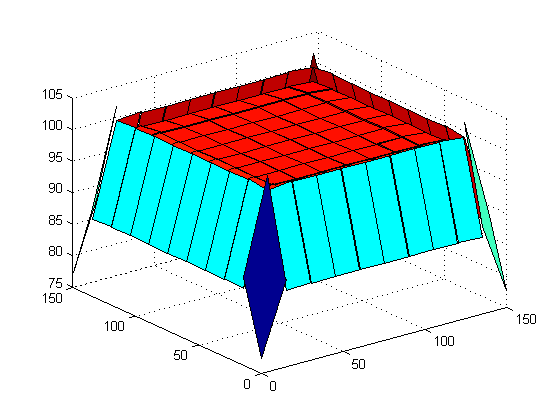
\includegraphics[scale=0.45]{IP10x10}
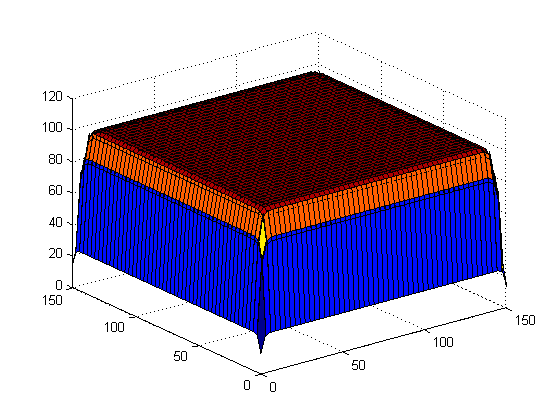
\includegraphics[scale=0.45]{IP50x50}
\end{center}
\caption{Solution of a diffusion equation based on the interior penalty method.}
\label{fig:ip}
\end{figure}
%%%%%%%%%%%%%%%%%%%%%%%%%%%%%%%%%%%%%%%%%%%%%%%%%%%%%%%%%%%%%%%%%%%%%%%%%%%%%%%%%%%%%%
%%%%%%%%%%%%%%%%%%%%%%%%%%%%%%%%%%%%%%%%%%%%%%%%%%%%%%%%%%%%%%%%%%%%%%%%%%%%%%%%%%%%%%
\Section{TRANSPORT SOLVES} \label{sec:transport}
%%%%%%%%%%%%%%%%%%%%%%%%%%%%%%%%%%%%%%%%%%%%%%%%%%%%%%%%%%%%%%%%%%%%%%%%%%%%%%%%%%%%%%
%%%%%%%%%%%%%%%%%%%%%%%%%%%%%%%%%%%%%%%%%%%%%%%%%%%%%%%%%%%%%%%%%%%%%%%%%%%%%%%%%%%%%%
The \sn transport equations (with isotropic source and scattering) are given by:
%
\begin{equation}
  \(\bo_d\cdot \bn + \Sigma_t(\br)\)\psi_d (\br) = \frac{1}{4\pi} \Sigma_s
  (\br) \phi(\br) + \frac{1}{4\pi} S (\br), \ \textrm{ for } \br \in \mc{D},\
  1 \leq d \leq M
  \label{transport_sn}
\end{equation}
with $\psi_d(\br) = \psi(\br,\bo_d)$ the angular flux at position $\br$ in
direction $\bo_d$, $\Sigma_t$ and $\Sigma_s$ the total and scattering cross
sections, respectively. The scalar flux is
defined as and evaluated as follows:
\begin{equation}
  \phi(\br) \equiv \int_{4\pi} \psi(\br,\bo) d\bo \approx \sum_{d=1}^M w_d
  \psi_d (\br).
\end{equation}
For brevity, we assume only incoming boundary conditions, $\psi_d(\br_b) =
\psi_d^{inc}(\br_b)$, for any boundary location $\br_b \in \partial \mc{D}_d^-
= \{\partial \mc{D} \textrm{ such that }\bo_d \cdot \bs{n}_b <0\}$, where
$\bs{n}_b = \bs{n}(\br_b)$ is the outward unit normal vector at the boundary. 
%
\eqt{transport_sn} can be written in a compact form using operators:
\begin{align}
  & \bs{L} \Psi = \bs{M \Sigma}\Phi + S \equiv q, \label{L_Psi}\\
  &\Phi = \bs{D} \Psi, \label{Phi}
\end{align}
%where $\Psi$ is the vector of angular fluxes, $\Phi$ the vector scalar flux,
%$q$ is the total (scattering+external) source $\bs{L}$ is the streaming
%operator, $\bs{M}$ is the moment-to-direction operator, and $\bs{D}$ is the
%direction-to-moment operator. $\bs{L} = diag
%(\bs{L}_1,\hdots,\bs{L}_d,\hdots,\bs{L}_M)$ is a diagonal operator; given a
%total cross section, one can solve independently for the resulting angular
%fluxes in all directions. The action of $\bs{L}^{-1}$ is often referred to as
%a \emph{transport sweep} when discontinuous spatial approximations are
%employed because, for any direction $\bo_d$, the action of $\bs{L}_d^{-1}$ can
%be obtained by traversing the mesh (i.e., sweeping) in a specific ordering of
%the cells, thus one needs only to solve a small linear system of equations,
%cell by cell. The order in which the elements are solved constitutes the graph
%of the sweep; for brevity and because this is not the focus of this article,
%we do not expand on situations where the graph can present some dependencies
%(cycles); in such a case, these dependencies can either be lagged within the
%iterative procedure or the solution vector consisting of the scalar flux is
%augmented by the angular fluxes that cause the cycle.

\eqt{L_Psi}--\eqt{Phi} can be solved using the Source Iteration (SI) method (a
stationary iterative technique also known as Richardson iteration). The SI
technique at the $\ell^{th}$ iteration is given by :
\begin{equation}
  \Phi^{(\ell+1)} = \bs{DL}^{-1} \(\bs{M\Sigma}\Phi^{(\ell)} + S\) .
\end{equation}
Alternatively, a subspace Krylov method (usually GMRes) can be employed to
solve the system of equations:
\begin{equation}
  \(\bs{I} - \bs{DL}^{-1}\bs{M \Sigma}\) \Phi = \bs{DL}^{-1}S .
\end{equation}
Both the SI and the GMRes approaches require transport sweeps (the action of
$\bs{L}^{-1}$ is required in both procedures).

When the scattering ratio $c=\frac{\Sigma_s}{\Sigma_t}$ tends to one in
optically thick domains, the number of SI and GMRes iterations can become large. To
accelerate the convergence, a DSA preconditioner is needed; the Modified IP
discontinuous finite element discretization of the diffusion equation for
rectangular grids is presented next.

%\subsection{Discontinuous Finite Element Discretization on Arbitrary Grids}
%
%The domain $\mc{D}$ is meshed into element $K$ (specifically polygons and
%polyhedra). For a given streaming direction $\bo_d$, the discontinuous finite
%element scheme on a given element $K$ is given by:
%\begin{equation}
  %-\int_{K} \(\psi_d \bo_d \cdot \bn b + \Sigma_t \Psi_d b \)\ d\br +
  %\int_{\partial K^+} \bo_d \cdot \bs{n} \Psi_d b\ d\br = \int_{K} qb\ d\br +
  %\int_{\partial K^{-}} |\bo_d \cdot \bs{n}| \psi_d^{\uparrow}b \ d\br
  %\label{transport_int}
%\end{equation}
%where $b$ represents a generic basis function, $\partial K^{-}$ is the inflow
%face of element $K$, $\partial K^{+}$ is the outflow face of element $K$. The
%angular flux values on an inflow face, denoted by $\psi_d^{\uparrow}$ in
%\cref{transport_int}, are taken from the upwind neighbor element of that face.


%%%%%%%%%%%%%%%%%%%%%%%%%%%%%%%%%%%%%%%%%%%%%%%%%%%%%%%%%%%%%%%%%%%%%%%%%%%%%%%%%%%%%%
%%%%%%%%%%%%%%%%%%%%%%%%%%%%%%%%%%%%%%%%%%%%%%%%%%%%%%%%%%%%%%%%%%%%%%%%%%%%%%%%%%%%%%
\Section{A BILINEAR DISCONTINUOUS DIFFUSION SYNTHETIC ACCELERATOR} \label{sec:mip}
%%%%%%%%%%%%%%%%%%%%%%%%%%%%%%%%%%%%%%%%%%%%%%%%%%%%%%%%%%%%%%%%%%%%%%%%%%%%%%%%%%%%%%
%%%%%%%%%%%%%%%%%%%%%%%%%%%%%%%%%%%%%%%%%%%%%%%%%%%%%%%%%%%%%%%%%%%%%%%%%%%%%%%%%%%%%%

The idea behind synthetic acceleration is that the error between the (yet
unknown) transport solution and the latest SI iterate can be estimated from a
computationally less expensive process, yielding a correction term to be added
to the latest iterate in order to improve the next iterate. In DSA, the
corrective scalar flux contribution is sought through the following
diffusion solve, where the volumetric source term is due to the difference between
successive iterates (and there are no surfacic source terms since the incoming angular flux was
fully determined in the transport equation, thus the error diffusion problem is should 
be written with a vacuum boundary condition):
\begin{equation}
  \bs{A}\ \delta \Phi = \bs{\Sigma}\(\Phi^{(\ell+1/2)} - \Phi^{(\ell)}\).
\end{equation}
In our case, the diffusion matrix $\bs{A}$ is exactly the one obtained from the bilinear form \eqt{eq:matrix-ip-form},
except for its penalty coefficient $\kappa_e^{IP}$ being changed to $\kappa_e^{MIP}$, given below: 
\begin{equation}
\kappa_e^{MIP} = \max \( \frac{1}{4}\, , \, \kappa_e^{IP} \) .
\end{equation}
In doing so, we followed \cite{mip} where the same modification of the penalty coefficient was performed 
for triangular meshes and the Fourier analyses revealed the stability of the scheme. 
Our Fourier analyses for BLD are given in the Results Section below.

Then, the next SI iterate is obtained as follows:
\begin{equation}
  \Phi^{(\ell+1)} = \Phi^{(\ell+1/2)}+\delta \Phi.
\end{equation}

Similarly, DSA can be obtained to precondition GMRes transport solves. The
final form of that system is:
\begin{equation}
  \(\bs{I} +\bs{A}^{-1} \bs{\Sigma}\)\(\bs{I}-\bs{DL}^{-1}\bs{M\Sigma}\) \Psi
  = \(\bs{I}+\bs{A}^{-1}\bs{\Sigma}\) \bs{DL}^{-1} S.
\end{equation}
Both approaches, SI+DSA or DSA-preconditioned GMRes, require a linear system
solve involving the diffusion matrix $\bs{A}$. Ideally, such a matrix should
be SPD (such that efficient techniques can be employed in its linear solve)
and easy to form (even on arbitrary grids).

Again, it is important to note that the preconditioned-SI and preconditioned GMRes systems 
require the solution of a linear system involving the diffusion matrix $\bs{A}$. This matrix is 
SPD and pCG or AMG techniques will be employed to solve such systems.


%%%%%%%%%%%%%%%%%%%%%%%%%%%%%%%%%%%%%%%%%%%%%%%%%%%%%%%%%%%%%%%%%%%%%%%%%%%%%%%%%%%%%%
%%%%%%%%%%%%%%%%%%%%%%%%%%%%%%%%%%%%%%%%%%%%%%%%%%%%%%%%%%%%%%%%%%%%%%%%%%%%%%%%%%%%%%
\Section{RESULTS} \label{sec:results}
%%%%%%%%%%%%%%%%%%%%%%%%%%%%%%%%%%%%%%%%%%%%%%%%%%%%%%%%%%%%%%%%%%%%%%%%%%%%%%%%%%%%%%
%%%%%%%%%%%%%%%%%%%%%%%%%%%%%%%%%%%%%%%%%%%%%%%%%%%%%%%%%%%%%%%%%%%%%%%%%%%%%%%%%%%%%%
In this Section, we first present some Fourier analysis results for the SI+DSA solution techniques
based on BLD discretizations of the transport and diffusion operators. Then, results from
the implementation of MIP as a DSA preconditioner in a BLD transport code are provided.

%%%%%%%%%%%%%%%%%%%%%%%%%%%%%%%%%%%%%%%%%%%%%%%%%%%%%%%%%%%%%%%%%%%%%%%%%%%%%%%%%%%%%%
\Subsection{Fourier Analyses for MIP-DSA using a BLD discretization} \label{sec:fourier}
%%%%%%%%%%%%%%%%%%%%%%%%%%%%%%%%%%%%%%%%%%%%%%%%%%%%%%%%%%%%%%%%%%%%%%%%%%%%%%%%%%%%%%
To analyze the performance of acceleration schemes, it is customary to carry out a Fourier Analysis (FA) on the discretized equations. A large body of work exists in the transport community regarding the application of FA to the study of acceleration of the SI scheme with DSA, both for the continuous and discretized equations \cite{consistent_p1}. Obviously, for numerical applications, the study of the discretized $\{$transport $+$ acceleration$\}$ solvers is of prime interest. Here, we employ a periodic homogeneous domain. In FA analysis, the error is decomposed into modes that are charactered by Fourier wave numbers. How these modes are damped during one step of the SI+DSA scheme provides insight on the effectiveness of the acceleration method. This damping is characterized by the spectral radius, the largest attenuation factor for any wave number. 
The slowest mode will dominate as the iteration proceeds and its damping rate, i.e., the largest attenuation factor for any wave number or spectral radius, will eventually characterize the iteration procedure.

\fig{fig:FA} presents the FA. The spectral radius is plotted as a function of the mesh optical thickness and the analysis are carried out for
$S_2$ through $S_{16}$. The spectral radius is always less than 0.65 (worst situation is for $S_2$, for $S_8$ and higher order \sn quadratures, the spectral radius is less than $\sim 0.4$). In the fine mesh limit, the standard results from the 2D continuous Fourier analysis (that is, continuous in the sense of ``not spatially discretized'') are recovered: the spectral radius for $S_2$ is $0.5c$ and, as $n$ increases, the spectral radius tends towards $0.2247c$. The results of \fig{fig:FA} are very similar to the ones obtained in \cite{mip} on 2D triangular meshes. 

\begin{figure}[!hbtp]
\begin{center}
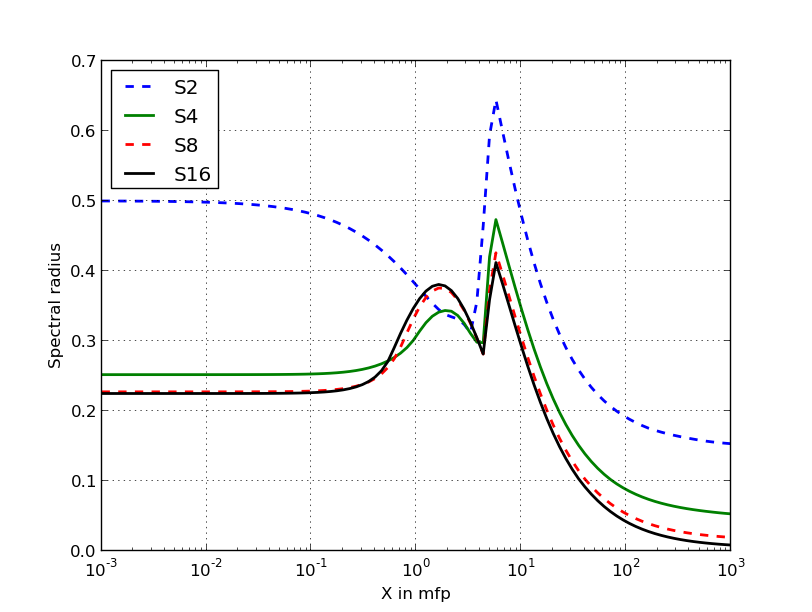
\includegraphics[scale=0.6]{optical_thickness_bld}
\end{center}
\caption{Fourier analysis for the MIP-DSA form as a function of the mesh optical thickness, homogeneous infinite medium case.}
\label{fig:FA}
\end{figure}

%%%%%%%%%%%%%%%%%%%%%%%%%%%%%%%%%%%%%%%%%%%%%%%%%%%%%%%%%%%%%%%%%%%%%%%%%%%%%%%%%%%%%%
\Subsection{Numerical Results} \label{sec:2d-results}
%%%%%%%%%%%%%%%%%%%%%%%%%%%%%%%%%%%%%%%%%%%%%%%%%%%%%%%%%%%%%%%%%%%%%%%%%%%%%%%%%%%%%%

The MIP-DSA technique has been implemented in  an \sn transport code using rectangular cells and BLD DFE basis functions. 
The following test cases were run: the domain is square $100cm \times 100cm$ with vacuum 
boundaries. There are 10000 cells and we use BLD finite elements; 
there are 40000 degrees of freedom. The relative tolerance on SI is $10^{-8}$ 
and the relative tolerance on CG is $10^{-10}$. We use a $S_{8}$ angular quadrature, 
$\Sigma_t = 1 cm^{-1}$, and $\Sigma_s = 0.999 cm^{-1}$. The source is uniform,
$1n/(cm^3s)$. In the first test, the domain is discretized using 100 cells along
$x$ and 100 cells along $y$. In the second test, the domain is discretized using
250 cells along $x$ and 40 cells along $y$; therefore, the aspect ratio is 6.25
for the second test. In the third test, the domain is discretized using 1000
cells along $x$ and 10 cells along $y$ (the aspect ratio is 100).

In \tbl{bld_ar_1}--\tbl{bld_ar_100}, we compare the CPU time and number of iterations for SI alone (no DSA), SI+DSA where the diffusion solves
are carried out using  unpreconditioned CG, and  SI+DSA where the diffusion solves
are carried out using  CG preconditioned with AMG.
In this Table, SI iter is the number of Source Iteration iterations 
needed to solve the problem, Prec is the time in seconds needed to
initialize the preconditioner used by CG, MIP is the total time in
seconds spent solving DSA during the calculation, CG iter is the total number 
of CG iterations used to solve MIP, and Total is the time in
seconds needed to solve the problem.
We note that solving the MIP equations requires more CG iterations when the aspect
ratio increases, but when preconditioned with AMG, CG remains very efficient. 

    \begin{table}[H]
\centering
      \caption{Comparison of preconditioners on rectangular mesh with an aspect ratio of 1.0 with BLD finite elements}
      \begin{tabular}{|c|c|c|c|c|c|c|c|c|}
        \hline
        & No-DSA & CG & AMG+CG \\
        \hline
        SI iter    & 7311    & 21      & 21      \\
        Prec (s)   & NA      & NA      & 0.057   \\
        MIP (s)    & NA      & 39.4564 & 2.76611 \\
        CG iter    & NA      & 8584    & 265     \\
        Total (s)  & 8254.46 & 66.8963 & 31.6606 \\
        \hline
      \end{tabular}
      \label{bld_ar_1}      
    \end{table}
    \begin{table}[H]
\centering
    \caption{Comparison of preconditioners on rectangular mesh with an aspect ratio of 6.25 with BLD finite elements}  
      \begin{tabular}{|c|c|c|c|c|c|c|c|c|}
        \hline
        & No-DSA & CG & AMG+CG \\
        \hline
        SI iter    & 7311    & 23      & 23      \\
        Prec (s)   & NA      & NA      & 0.671   \\
        MIP (s)    & NA      & 87.8195 & 4.20011 \\
        CG iter    & NA      & 18985   & 171     \\
        Total (s)  & 7311.49 & 117.768 & 32.857  \\
        \hline
      \end{tabular}
      \label{bld_ar_6}      
    \end{table}
    \begin{table}[H]
\centering
    \caption{Comparison of preconditioners on rectangular mesh with an aspect ratio of 100 with BLD finite elements}  
      \begin{tabular}{|c|c|c|c|c|c|c|c|c|}
        \hline
        & No-DSA & CG & AMG+CG \\
        \hline
        SI iter    & 7304    & 24      & 24      \\
        Prec (s)   & NA      & NA      & 0.383   \\
        MIP (s)    & NA      & 361.306 & 3.74259 \\
        CG iter    & NA      & 82613   & 177     \\
        Total (s)  & 8581.25 & 400.116 & 43.6815 \\
        \hline
      \end{tabular}
      \label{bld_ar_100}      
    \end{table}
%%%%%%%%%%%%%%%%%%%%%%%%%%%%%%%%%%%%%%%%%%%%%%%%%%%%%%%%%%%%%%%%%%%%%%%%%%%%%%%%%%%%%%
%%%%%%%%%%%%%%%%%%%%%%%%%%%%%%%%%%%%%%%%%%%%%%%%%%%%%%%%%%%%%%%%%%%%%%%%%%%%%%%%%%%%%%
\Section{CONCLUSIONS AND OUTLOOK} \label{sec:ccl}
%%%%%%%%%%%%%%%%%%%%%%%%%%%%%%%%%%%%%%%%%%%%%%%%%%%%%%%%%%%%%%%%%%%%%%%%%%%%%%%%%%%%%%
%%%%%%%%%%%%%%%%%%%%%%%%%%%%%%%%%%%%%%%%%%%%%%%%%%%%%%%%%%%%%%%%%%%%%%%%%%%%%%%%%%%%%%

A discontinuous finite element technique based on the interior penalty method was used to
solve the DSA equations in $xy$ rectangular cells using BLD basis functions. 
Fourier analysis results show that the technique is stable and efficient, with a spectral
radius of $\sim 0.4$ for $S_*$ and higher angular \sn quadratures. The discretized diffusion 
equations are SPD and thus are amenable to preconditioned CG linear solvers (we employed an
algebraic multigrid technique). The scheme was found to be very efficient, even for problems 
with cells presenting aspect ratios as high as 100.

In the future, we plan to extend this MPI-DSA technique to the PieceWise Linear Discontinuous (PWLD) technique
for arbitrary polygons. 
%%%%%%%%%%%%%%%%%%%%%%%%%%%%%%%%%%%%%%%%%%%%%%%%%%%%%%%%%%%%%%%%%%%%%%%%%%%%%%%%%%%%%%
%%%%%%%%%%%%%%%%%%%%%%%%%%%%%%%%%%%%%%%%%%%%%%%%%%%%%%%%%%%%%%%%%%%%%%%%%%%%%%%%%%%%%%
\Section{APPENDIX} \label{sec:app}
%%%%%%%%%%%%%%%%%%%%%%%%%%%%%%%%%%%%%%%%%%%%%%%%%%%%%%%%%%%%%%%%%%%%%%%%%%%%%%%%%%%%%%
%%%%%%%%%%%%%%%%%%%%%%%%%%%%%%%%%%%%%%%%%%%%%%%%%%%%%%%%%%%%%%%%%%%%%%%%%%%%%%%%%%%%%%

For completeness, the elementary matrices needed to assemble the global matrix corresponding to the
bilinear form \eqt{eq:matrix-ip-form} are given below. The BLD basis functions $\( \tf_{k} \)_{1 \le k \le 4}$
were given earlier, in Section~\ref{sec:ip}. 

Matrices' names that are \underline{{\bf underlined and bold}} are elementary matrices not present in the DFEM
discretization of the transport equation. All other elementary matrices are already present in the transport discretization.

The {\bf mass matrix} is given by :
\begin{equation}
M = \frac{{\Delta _x}{\Delta _y}}{36}
\begin{pmatrix}
4 & 2 & 1 & 2 \\
2 & 4 & 2 & 1 \\
1 & 2 & 4 & 2 \\
2 & 1 & 2 & 4 
\end{pmatrix}
\end{equation}
The {\bf gradient matrix ($\partial_x$)} is given by :
\begin{equation}
\int \tf_i \frac{\partial \tf_j}{\partial x} d\br = \frac{{\Delta _y}}{12}
\begin{pmatrix}
 -2 & -2 & -1 & -1 \\
  2 &  2 &  1 &  1\\
  1 &  1 &  2 &  2\\
 -1 & -1 & -2 & -2
\end{pmatrix}
\end{equation}
The {\bf gradient matrix ($\partial_y$)} is given by :
\begin{equation}
\int \tf_i \frac{\partial \tf_j}{\partial y} d\br = \frac{{\Delta _x}}{12}
\begin{pmatrix}
 -2 & -1 & -1 & -2 \\
 -1 & -2 & -2 & -1\\
  1 &  2 &  2 &  1\\
  2 &  1 &  1 &  2
\end{pmatrix}
\end{equation}
The \underline{{\bf stiffness matrix}} is given by :
\begin{equation}
S = \frac{{\Delta _y}}{6{\Delta _x}}
\begin{pmatrix}
2 & -2 & -1 & 1 \\
-2 & 2 & 1 & -1 \\
-1 & 1 & 2 & -2 \\
1 & -1 & -2 & 2 
\end{pmatrix}
+ \frac{{\Delta _x}}{6{\Delta _y}}
\begin{pmatrix}
2 & 1 & -1 & -2 \\
1 & 2 & -2 & -1 \\
-1 & -2 & 2 & 1 \\
-2 & -1 & 1 & 2 
\end{pmatrix}
\end{equation}
The {\bf horizontal edge mass matrix} (e.g., for angular flux upwinding on outgoing edge) is given by :
\begin{equation}
E_{M,h} = \frac{{\Delta _x}}{6}
\begin{pmatrix}
2 & 1 \\
1 & 2 
\end{pmatrix}
\end{equation}
The {\bf horizontal coupling edge mass matrix} (e.g., for angular flux upwinding on incoming edge) is given by :
\begin{equation}
E_{M,h}^c = \frac{{\Delta _x}}{6}
\begin{pmatrix}
1 & 2 \\
2 & 1 \\
\end{pmatrix}
\end{equation}
The {\bf vertical edge mass matrix} is given by :
\begin{equation}
E_{M,v} = \frac{{\Delta _y}}{6}
\begin{pmatrix}
2 & 1\\
1 & 2
\end{pmatrix}
\end{equation}
The {\bf vertical coupling edge mass matrix} is given by :
\begin{equation}
E_{M,v}^c = \frac{{\Delta _y}}{6}
\begin{pmatrix}
2 & 1 \\
1 & 2 \\
\end{pmatrix}
\end{equation}
The {\bf gradient edge mass matrix} $(\tf,\partial_{\bs{n}}
\tf)_{E_h^i}=\(\partial_{\bs{n}}\tf,\tf\)_{E_h^i}^T$ :
\begin{itemize}
\item {\bf left edge} (right, top and bottom edge gradient coupling matrices are obtained in a similar manner)  %(assumed $\bs{n}\cdot\bs{1}_x = 1$)
\begin{equation}
\begin{split}
\int_{0}^{{\Delta _y}} \partial_x \tf^{T} \cdot \tf\ dy &= \int_0^{\Delta _y}
\begin{pmatrix}
-\frac{1}{{\Delta _x}}\frac{{\Delta _y}-y}{{\Delta _y}}\\
\frac{1}{{\Delta _x}} \frac{{\Delta _y}-y}{{\Delta _y}}\\
\frac{1}{{\Delta _x}} \frac{y}{{\Delta _y}}\\
-\frac{1}{{\Delta _x}} \frac{y}{{\Delta _y}}
\end{pmatrix}
\cdot
\begin{pmatrix}
\frac{{\Delta _y}-y}{{\Delta _y}} & 0 & 0 & \frac{y}{{\Delta _y}}
\end{pmatrix}
dy\\
&= \int_0^{\Delta _y} 
\begin{pmatrix}
-\frac{1}{{\Delta _x}} \(\frac{{\Delta _y}-y}{{\Delta _y}}\)^2 & 0 & 0 & -\frac{1}{{\Delta _x}} \frac{{\Delta _y}y-y^2}{{\Delta _y}^2} \\
\frac{1}{{\Delta _x}} \(\frac{{\Delta _y}-y}{{\Delta _y}}\)^2  & 0 & 0 & \frac{1}{{\Delta _x}} \frac{{\Delta _y}y-y^2}{{\Delta _y}^2}\\
\frac{1}{a} \frac{{\Delta _y}y-y^2}{{\Delta _y}^2}   & 0 & 0 & \frac{1}{a} \(\frac{y}{{\Delta _y}}\)^2 \\
-\frac{1}{a} \frac{{\Delta _y}y-y^2}{{\Delta _y}^2}  & 0 & 0 & -\frac{1}{a} \(\frac{y}{{\Delta _y}}\)^2
\end{pmatrix}
dy\\
&= 
\begin{pmatrix}
-\frac{{\Delta _y}}{3{\Delta _x}} & 0 & 0 & -\frac{{\Delta _y}}{6{\Delta _x}} \\
\frac{{\Delta _y}}{3{\Delta _x}} & 0 & 0 & \frac{{\Delta _y}}{6{\Delta _x}} \\
\frac{{\Delta _y}}{6{\Delta _x}} & 0 & 0 & \frac{{\Delta _y}}{3{\Delta _x}} \\
-\frac{{\Delta _y}}{6{\Delta _x}} & 0 & 0 & -\frac{{\Delta _y}}{3{\Delta _x}}
\end{pmatrix}\\
& = \frac{{\Delta _y}}{6{\Delta _x}}
\begin{pmatrix}
-2 & 0 & 0 & -1 \\
2 & 0 & 0 & 1 \\
1 & 0 & 0 & 2 \\
-1 & 0 & 0 & -2
\end{pmatrix}
\end{split}
\end{equation}
%\item {\bf right edge} (assumed $\bs{n}\cdot\bs{1}_x = 1$)
%\begin{equation}
%\begin{split}
%\int_0^{\Delta _y} \partial_x \tf^{T} \cdot \tf\ dy &= 
%\int_0^{\Delta _y} 
%\begin{pmatrix}
%-\frac{1}{{\Delta _x}} \frac{{\Delta _y}-y}{{\Delta _y}} \\
%\frac{1}{{\Delta _x}} \frac{{\Delta _y}-y}{{\Delta _y}}  \\
%\frac{1}{{\Delta _x}} \frac{y}{{\Delta _y}}    \\
%-\frac{1}{{\Delta _x}} \frac{y}{{\Delta _y}}   
%\end{pmatrix}
%\cdot
%\begin{pmatrix}
%0 & \frac{{\Delta _y}-y}{{\Delta _y}} & \frac{y}{{\Delta _y}} & 0
%\end{pmatrix}
%dy\\
%&= \int_0^{\Delta _y} 
%\begin{pmatrix}
%0 & -\frac{1}{{\Delta _x}} \(\frac{{\Delta _y}-y}{{\Delta _y}}\)^2 & -\frac{1}{{\Delta _x}} \frac{{\Delta _y}y-y^2}{{\Delta _y}^2} & 0 \\
%0 & \frac{1}{{\Delta _x}} \(\frac{{\Delta _y}-y}{{\Delta _y}}\)^2 & \frac{1}{{\Delta _x}} \frac{{\Delta _y}y-y^2}{{\Delta _y}^2} & 0 \\
%0 & \frac{1}{{\Delta _x}} \frac{{\Delta _y}y-y^2}{{\Delta _y}^2} & \frac{1}{{\Delta _x}} \(\frac{y}{{\Delta _y}}\)^2 & 0 \\
%0 & -\frac{1}{{\Delta _x}} \frac{{\Delta _y}y-y^2}{{\Delta _y}^2} & -\frac{1}{{\Delta _x}} \(\frac{y}{{\Delta _y}}\)^2 & 0 
%\end{pmatrix}
%dy \\
%&=
%\begin{pmatrix}
 %0 & -\frac{{\Delta _y}}{3{\Delta _x}} & -\frac{{\Delta _y}}{6{\Delta _x}} & 0 \\
 %0 & \frac{{\Delta _y}}{3{\Delta _x}} & \frac{{\Delta _y}}{6{\Delta _x}} & 0 \\
 %0 & \frac{{\Delta _y}}{6{\Delta _x}} & \frac{{\Delta _y}}{3{\Delta _x}} & 0 \\
 %0 & -\frac{{\Delta _y}}{6{\Delta _x}} & -\frac{{\Delta _y}}{3{\Delta _x}} & 0 
%\end{pmatrix}\\
%&=\frac{{\Delta _y}}{6{\Delta _x}}
%\begin{pmatrix}
%0 & -2 & -1 & 0 \\
%0 & 2 & 1 & 0 \\
%0 & 1 & 2 & 0 \\
%0 & -1 & -2 & 0
%\end{pmatrix}
%\end{split}
%\end{equation}
%\item {\bf bottom edge} (assumed $\bs{n}\cdot\bs{1}_x = -1$)
%\begin{equation}
%\begin{split}
%\int_0^{\Delta _x} \partial_y \tf^{T} \cdot \tf\ dx &= \int_0^{\Delta _x}
%\begin{pmatrix}
%-\frac{1}{{\Delta _y}} \frac{{\Delta _x}-x}{{\Delta _x}} \\
%-\frac{1}{{\Delta _y}} \frac{x}{{\Delta _x}} \\
%\frac{1}{{\Delta _y}} \frac{x}{{\Delta _x}} \\
%\frac{1}{{\Delta _y}} \frac{{\Delta _x}-x}{{\Delta _x}} 
%\end{pmatrix}
%\cdot
%\begin{pmatrix}
%\frac{{\Delta _x}-x}{{\Delta _x}} & \frac{x}{{\Delta _x}} & 0 & 0
%\end{pmatrix}
%dx \\
%& = \int_0^{\Delta _x} 
%\begin{pmatrix}
%-\frac{1}{{\Delta _y}}\(\frac{{\Delta _x}-x}{{\Delta _x}}\)^2 & -\frac{1}{{\Delta _y}} \frac{{\Delta _x}x-x^2}{{\Delta _x}^2} & 0 & 0 \\
%-\frac{1}{{\Delta _y}}\frac{{\Delta _x}x-x^2}{{\Delta _x}^2} & -\frac{1}{{\Delta _y}} \(\frac{x}{{\Delta _x}}\)^2 & 0 & 0 \\
%\frac{1}{{\Delta _y}} \frac{{\Delta _x}x-x^2}{{\Delta _x}^2} & \frac{1}{{\Delta _y}}\(\frac{x}{{\Delta _x}}\)^2 & 0 & 0 \\
%\frac{1}{{\Delta _y}} \(\frac{{\Delta _x}-x}{{\Delta _x}}\)^2 & \frac{1}{{\Delta _y}}\frac{{\Delta _x}x-x^2}{{\Delta _x}^2} & 0 & 0
%\end{pmatrix}
%dx\\
%&= 
%\begin{pmatrix}
%-\frac{{\Delta _x}}{3{\Delta _y}} & -\frac{{\Delta _x}}{6{\Delta _y}} & 0 & 0 \\
%-\frac{{\Delta _x}}{6{\Delta _y}} & -\frac{{\Delta _x}}{3{\Delta _y}} & 0 & 0 \\
%\frac{{\Delta _x}}{6{\Delta _y}} & \frac{{\Delta _x}}{3{\Delta _y}} & 0 & 0 \\
%\frac{{\Delta _x}}{3{\Delta _y}} & \frac{{\Delta _x}}{6{\Delta _y}} & 0 & 0 
%\end{pmatrix}\\
%&= \frac{{\Delta _x}}{6{\Delta _y}} 
%\begin{pmatrix}
%-2 & -1 & 0 & 0 \\
%-1 & -2 & 0 & 0 \\
%1 & 2 & 0 & 0 \\
%2 & 1 & 0 & 0
%\end{pmatrix}
%\end{split}
%\end{equation}
%\item {\bf top edge} (assumed $\bs{n}\cdot \bs{1}_x = 1$)
%\begin{equation}
%\begin{split}
%\int_0^{\Delta _x} \partial_y \tf^{T}\cdot \tf\ dx &= \int_0^{\Delta _x} 
%\begin{pmatrix}
%-\frac{1}{{\Delta _y}} \frac{{\Delta _x}-x}{{\Delta _x}} \\
%-\frac{1}{{\Delta _y}} \frac{x}{{\Delta _x}} \\
%\frac{1}{{\Delta _y}} \frac{x}{{\Delta _x}} \\
%\frac{1}{{\Delta _y}} \frac{{\Delta _x}-x}{{\Delta _x}}
%\end{pmatrix}
%\cdot
%\begin{pmatrix}
%0 & 0 & \frac{x}{{\Delta _x}} & \frac{{\Delta _x}-x}{{\Delta _x}}
%\end{pmatrix}
%dx\\
%&=\int_0^{\Delta _x} 
%\begin{pmatrix}
%0 & 0 & -\frac{1}{{\Delta _y}}\frac{{\Delta _x}x-x^2}{a^2} & -\frac{1}{{\Delta _y}} \(\frac{{\Delta _x}-x}{{\Delta _x}}\)^2 \\
%0 & 0 & -\frac{1}{{\Delta _y}}\(\frac{x}{{\Delta _x}}\)^2 & -\frac{1}{{\Delta _y}} \frac{{\Delta _x}x-x^2}{{\Delta _x}^2} \\
%0 & 0 & \frac{1}{{\Delta _y}}\(\frac{x}{{\Delta _x}}\)^2 & \frac{1}{{\Delta _y}} \frac{{\Delta _x}x-x^2}{{\Delta _x}^2} \\
%0 & 0 & \frac{1}{{\Delta _y}}\frac{{\Delta _x}x-x^2}{{\Delta _x}} & \frac{1}{{\Delta _y}}\(\frac{{\Delta _x}-x}{{\Delta _x}}\)^2
%\end{pmatrix}
%dx\\
%&= 
%\begin{pmatrix}
%0 & 0 & -\frac{{\Delta _x}}{6{\Delta _y}} & -\frac{{\Delta _x}}{3{\Delta _y}} \\
%0 & 0 & -\frac{{\Delta _x}}{3{\Delta _y}} & -\frac{{\Delta _x}}{6{\Delta _y}} \\
%0 & 0 & \frac{{\Delta _x}}{3{\Delta _y}} & \frac{{\Delta _x}}{6{\Delta _y}} \\
%0 & 0 & \frac{{\Delta _x}}{6{\Delta _y}} & \frac{{\Delta _x}}{3{\Delta _y}} 
%\end{pmatrix}\\
%&= \frac{{\Delta _x}}{6{\Delta _y}}
%\begin{pmatrix}
%0 & 0 & -1 & -2 \\
%0 & 0 & -2 & -1 \\
%0 & 0 & 2 & 1 \\
%0 & 0 & 1 & 2
%\end{pmatrix}
%\end{split}
%\end{equation}
\end{itemize}
The {\bf gradient coupling-edge mass matrix}
$(\tf^{\pm},\partial_{\bs{n}}\tf^{\pm})_{E_h^i}$ and
$(\partial_{\bs{n}}\tf^{\pm},\tf^{\pm})_{E_h^i}$ :
\begin{itemize}
\item {\bf vertical edge} (right, top and bottom edge gradient coupling matrices are obtained in a similar manner)  %(assumed $\bs{n}\cdot \bs{1}_x =1$) :
\begin{equation}
\begin{split}
\(\tf^-,\partial_x \tf^{+}\)_{E_h^i} & = \int_0^{\Delta _y} \partial_x \tf^{+,T}\cdot
\tf^-\ dy\\
&= \int_0^{\Delta _y}
\begin{pmatrix}
-\frac{1}{{\Delta _x}^+} \frac{{\Delta _y}-y}{{\Delta _y}} \\
\frac{1}{{\Delta _x}^+} \frac{{\Delta _y}-y}{{\Delta _y}} \\
\frac{1}{{\Delta _x}^+} \frac{y}{{\Delta _y}} \\
-\frac{1}{{\Delta _x}^+} \frac{y}{{\Delta _y}} 
\end{pmatrix}
\cdot
\begin{pmatrix}
0 & \frac{{\Delta _y}-y}{{\Delta _y}} & \frac{y}{{\Delta _y}} & 0
\end{pmatrix}\\
&= \frac{{\Delta _y}}{6{\Delta _x}^+}
\begin{pmatrix}
0 & -2 & -1 & 0 \\
0 & 2 & 1 & 0 \\
0 & 1 & 2 & 0 \\
0 & -1 & -2 & 0
\end{pmatrix}
\end{split}
\end{equation}
\begin{equation}
\begin{split}
\(\tf^+,\partial_x \tf^{-}\)_{E_h^i} &= \int_0^{{\Delta _y}} \partial_x \tf^{-,T}\cdot
\tf^+\ dy\\
& = \int_0^{\Delta _y} 
\begin{pmatrix}
-\frac{1}{{\Delta _x}^-} \frac{{\Delta _y}-y}{{\Delta _y}} \\
\frac{1}{{\Delta _x}^-} \frac{{\Delta _y}-y}{{\Delta _y}} \\
\frac{1}{{\Delta _x}^-} \frac{y}{{\Delta _y}} \\
-\frac{1}{{\Delta _x}^-} \frac{y}{{\Delta _y}}
\end{pmatrix}
\cdot
\begin{pmatrix}
\frac{{\Delta _y}-y}{{\Delta _y}} & 0 & 0 & \frac{y}{{\Delta _y}}
\end{pmatrix}
dy\\
&= \frac{{\Delta _y}}{6{\Delta _x}^-} 
\begin{pmatrix}
-2 & 0 & 0 & -1 \\
2 & 0 & 0 & 1 \\
1 & 0 & 0 & 2 \\
-1 & 0 & 0 & -2
\end{pmatrix}
\end{split}
\end{equation}
\begin{equation}
\begin{split}
\(\partial_x \tf^{+},\tf^{-}\)_{E_h^i} &= \int_0^{\Delta _y} \tf^{-,T} \cdot
\partial_x \tf^{+} dy\\
&= \int_0^{\Delta _y} 
\begin{pmatrix}
0 \\
\frac{{\Delta _y}-y}{{\Delta _y}} \\
\frac{y}{{\Delta _y}} \\
0
\end{pmatrix}
\cdot
\begin{pmatrix}
-\frac{1}{{\Delta _x}^+}\frac{{\Delta _y}-y}{{\Delta _y}} & \frac{1}{{\Delta _x}^+} \frac{{\Delta _y}-y}{{\Delta _y}} & \frac{1}{{\Delta _x}^+}
\frac{y}{{\Delta _y}} & -\frac{1}{{\Delta _x}^+} \frac{y}{{\Delta _y}} 
\end{pmatrix}
dy\\
&= \frac{{\Delta _y}}{6{\Delta _x}^+}
\begin{pmatrix}
0 & 0 & 0 & 0 \\
-2 & 2 & 1 & -1 \\
-1 & 1 & 2 & -2 \\
0 & 0 & 0 & 0
\end{pmatrix}
\end{split}
\end{equation}
\begin{equation}
\begin{split}
\(\partial_x \tf^-,\phi^{+}\)_{E_h^i} &= \int_0^{\Delta _y} \tf^{+,T}\cdot \partial_x
\tf^{-} dy\\
&=\int_0^{\Delta _y}
\begin{pmatrix}
\frac{{\Delta _y}-y}{{\Delta _y}}\\
0 \\
0 \\
\frac{y}{{\Delta _y}}
\end{pmatrix}
\cdot
\begin{pmatrix}
-\frac{1}{{\Delta _x}^-}\frac{{\Delta _y}-y}{{\Delta _y}} & \frac{1}{{\Delta _x}^-} \frac{{\Delta _y}-y}{{\Delta _y}} & \frac{1}{{\Delta _x}^-}
\frac{y}{{\Delta _y}} & -\frac{1}{{\Delta _x}^-}\frac{y}{{\Delta _y}}
\end{pmatrix}
dy\\
&= \frac{{\Delta _y}}{6{\Delta _x}^-}
\begin{pmatrix}
-2 & 2 & 1 & -1 \\
0 & 0 & 0 & 0 \\
0 & 0 & 0 & 0 \\
-1 & 1 & 2 & -2
\end{pmatrix}
\end{split}
\end{equation}
%
%\item {\bf horizontal edge} (assumed $\bs{n}\cdot\bs{1}_y =1$) :
%\begin{equation}
%\begin{split}
%(\tf^-,\partial_y \tf^{+})_{E_h^i} &= \int_0^{\Delta _x} \partial_y \tf^{+,T} \cdot
%\tf^{-} dx\\
%&= \frac{{\Delta _x}}{6{\Delta _y}^+}
%\begin{pmatrix}
%0 & 0 & -1 & -2 \\
%0 & 0 & -2 & -1 \\
%0 & 0 & 2 & 1 \\
%0 & 0 & 1 & 2
%\end{pmatrix}
%\end{split}
%\end{equation}
%\begin{equation}
%\begin{split}
%\(\tf^+,\partial_y \tf^{-}\)_{E_h^i} &= \int_0^{\Delta _x} \partial_y
%\tf^{-,T}\cdot \tf^+ dx\\
%&= \frac{{\Delta _x}}{6{\Delta _y}^-}
%\begin{pmatrix}
%-2 & -1 & 0 & 0 \\
%-1 & -2 & 0 & 0 \\
%1 & 2 & 0 & 0 \\
%2 & 1 & 0 & 0 
%\end{pmatrix}
%\end{split}
%\end{equation}
%\begin{equation}
%\begin{split}
%(\partial_y \tf^+, \tf^{-})_{E_h^i} &= \int_0^{\Delta _x} \tf^{-,T}\cdot \partial_y
%\tf^+\ dy\\
%&= \frac{{\Delta _x}}{6{\Delta _y}^-}
%\begin{pmatrix}
%0 & 0 & 0 & 0 \\
%0 & 0 & 0 & 0 \\
%-1 & -2 & 2 & 1 \\
%-2 & -1 & 1 & 2
%\end{pmatrix}
%\end{split}
%\end{equation}
%\begin{equation}
%\begin{split}
%(\partial_y\tf^-,\tf^{+})_{E_h^i} &= \int_0^{\Delta _x} \tf^{+,T}\cdot \partial_y
%\tf^- dy\\
%&= \frac{{\Delta _x}}{6{\Delta _y}^-}
%\begin{pmatrix}
%-2 & -1 & 1 & 2 \\
%-1 & -2 & 2 & 1 \\
%0 & 0 & 0 & 0 \\
%0 & 0 & 0 & 0
%\end{pmatrix}
%\end{split}
%\end{equation}
\end{itemize}



%\begin{table}[!htb]
%\centering
%\caption{\bf Parallel Performance for the Sample Problem}
%\label{table:example} 
%\vspace{14pt}
%\begin{tabular}{||r||c|c|c||} \hline \hline
 %\multicolumn{1}{||c||}{Number of} &
 %\multicolumn{1}{c|}{Wall-Clock} &
 %\multicolumn{1}{c|}{Speedup} &
 %\multicolumn{1}{c||}{Efficiency} \\
 %\multicolumn{1}{||c||}{Processors} &
 %\multicolumn{1}{c|}{Time$^{a}$ (min)} &
 %\multicolumn{1}{c|}{(T$_{s}$/T$_{p}$)} &
 %\multicolumn{1}{c||}{(\%)} \\ \hline\hline
%\ 1 &  100.0 & \ ---    & ---  \\ \hline
%\ 2 &   52.6 & \ 1.9    & 95.0 \\ \hline \hline
%\end{tabular}
%\end{table}

%\Section*{REFERENCES}
\setlength{\baselineskip}{12pt}
\begin{thebibliography}{300}

\bibitem{dsa_ref}
Marvin~L. Adams and Edward~W. Larsen.
\newblock {Fast iterative methods for discrete-ordinates particle transport
  calculations}.
\newblock {\em Progress in Nuclear Energy}, 40:3--159, 2002.

\bibitem{Kanschat2007}
Guido Kanschat.
\newblock {\em {Discontinuous Galerkin Methods for Viscous Incompressible
  Flow}}.
\newblock Springer, first edition, 2007.

\bibitem{larsen_dsa}
E.~W. Larsen.
\newblock {Diffusion-Synthetic Acceleration Methods for Discrete-Ordinates
  Problems}.
\newblock {\em Transport Theory and Statistical Physics}, 13:107--126, 1984.

\bibitem{mip}
Y.~Wang and J.C. Ragusa.
\newblock {Diffusion Synthetic Acceleration for High-Order Discontinuous Finite
  Element $S_n$ Transport Schemes and Application to Locally Refined
  Unstructured Meshes}.
\newblock {\em Nuclear Science and Engineering}, 166:145--166, 2010.

\bibitem{wla}
T.~A. Wareing, E.~W. Larsen, and M.~L. Adams.
\newblock {Diffusion Accelerated Discontinuous Finite Element Schemes for the
  Sn Equations in Slab and X-Y Geometries}.
\newblock {\em Proc. Int. Topl. Mtg. Adavances in Mathematics, Computations,
  and Reactor Physics, Pittsburgh, Pennsylvania}, April 28 - May 2 1991.
	
\bibitem{consistent_p1}
James~S. Warsa, Todd~A. Wareing, and Jim~E. Morel.
\newblock {Fully Consistent Diffusion Synthetic Acceleration of Linear
  Discontinuous $S_N$ Transport Discretizations on Unstructured Tetrahedral
  Meshes}.
\newblock {\em Nuclear Science and Engineering}, 141(3):236--251, July 2002.

\bibitem{nitsche}
J.~Nitsche.
\newblock {\"U}ber ein {V}ariationsprinzip zur {L\"o}sung von
  {D}irichlet-{P}roblemen bei der {V}erwendung von {T}eilr{\"a}umen, die keinen
  {R}andbedingungen unterworfen sind.
\newblock {\em Abh. Math. Univ. Hamburg}, 36:9--15, 1971.

\bibitem{ip-review}
Douglas N. Arnold, Franco Brezzi, Bernardo Cockburn, L. Donatella Marini
\newblock Unified Analysis Of Discontinuous Galerkin Methods For Elliptic Problems
\newblock {\em Siam J. Numer. Anal. }, Vol. 39, No. 5, Pp. 1749–1779, 2002

\end{thebibliography}

\end{document}


